\section{Dataset clusters comparison}

		\begin{figure*}[ht!]
			\centering
			\subfloat[Zernike coefficients]{%
				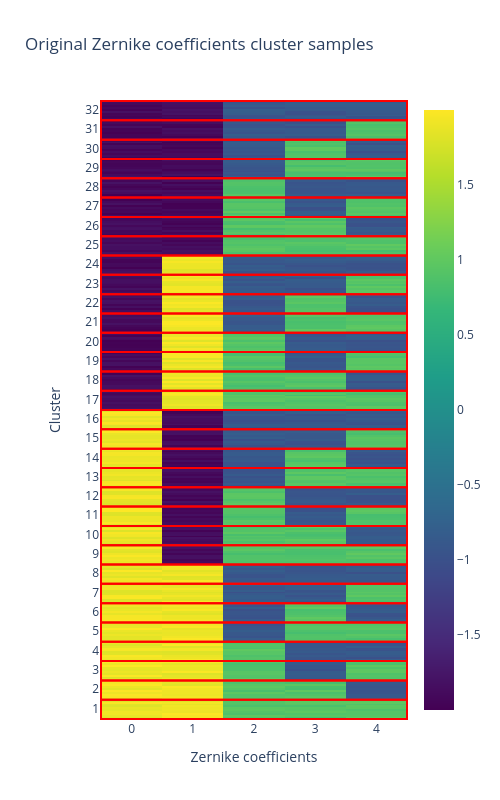
\includegraphics[width=0.22\textwidth]{mdid-5mzernikecoefficientsoriginalgridclusters.png}}
			\hspace{\fill}
			\subfloat[LP coefficients]{%
				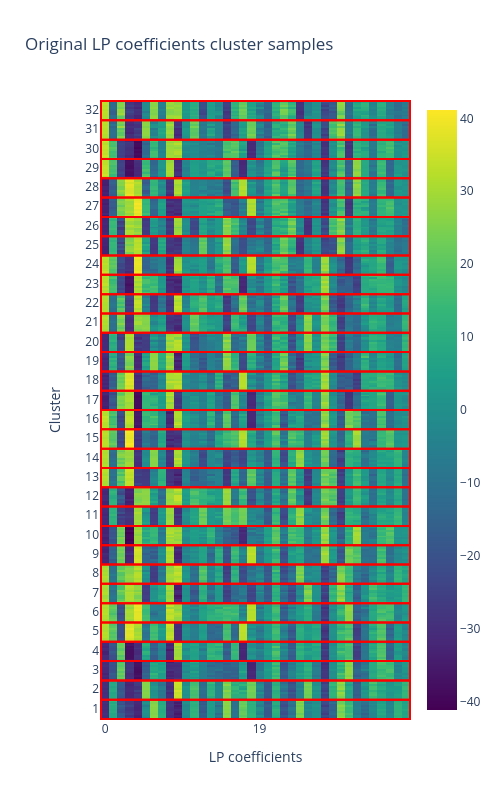
\includegraphics[width=0.22\textwidth]{mdid-5mlpcoefficientsoriginalgridclusters.png}}
			\hspace{\fill}
			\subfloat[Output fluxes]{%
				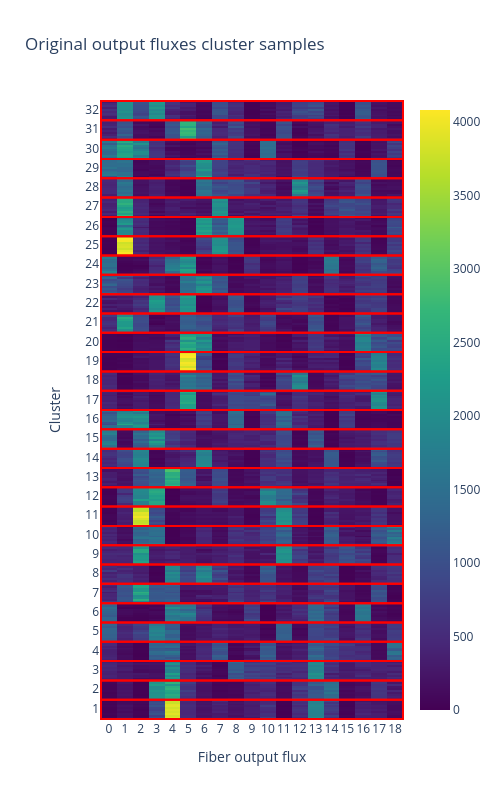
\includegraphics[width=0.22\textwidth]{mdid-5moutputfluxesoriginalgridclusters.png}}
			\hspace{\fill}
			\subfloat[PCA PSF Intensities]{%
				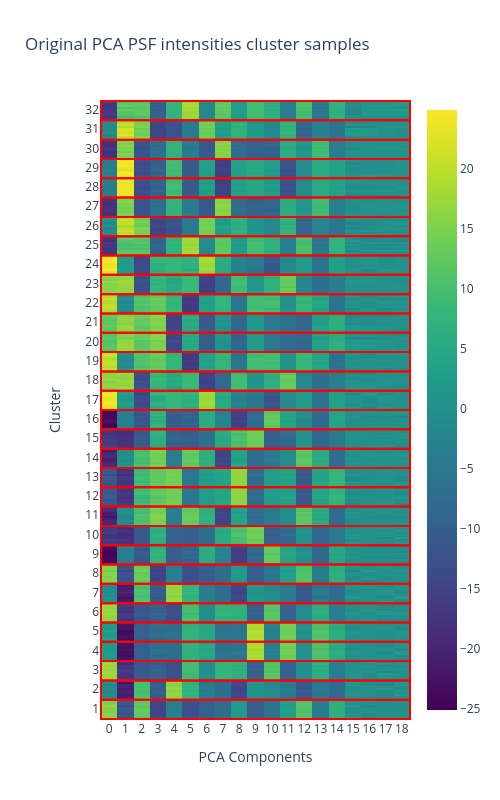
\includegraphics[width=0.22\textwidth]{mdid-5mpcaintensitiesoriginalgridclusters.png}}
			\hspace{\fill}
			\caption{Original clusters from the datasets}
		\end{figure*}
		\FloatBarrier
		
		\begin{figure*}[ht!]
			\centering
			\subfloat[Zernike coefficients]{%
				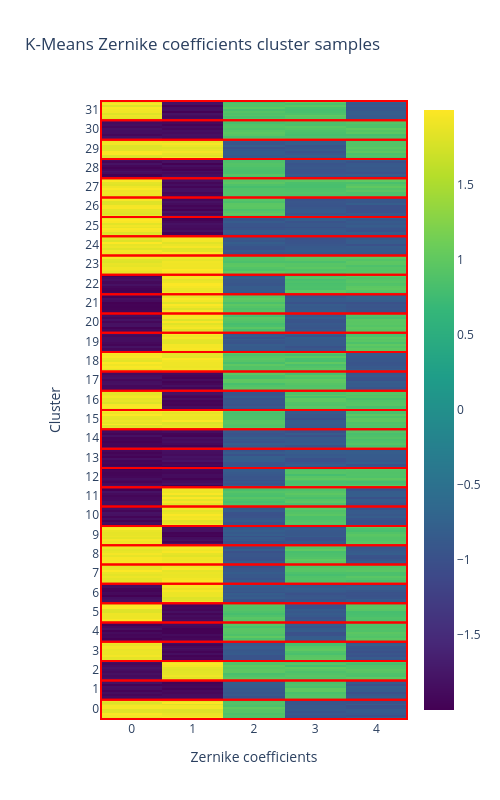
\includegraphics[width=0.22\textwidth]{mdid-5mzernikecoefficientsK-Meansgridclusters.png}}
			\hspace{\fill}
			\subfloat[LP coefficients]{%
				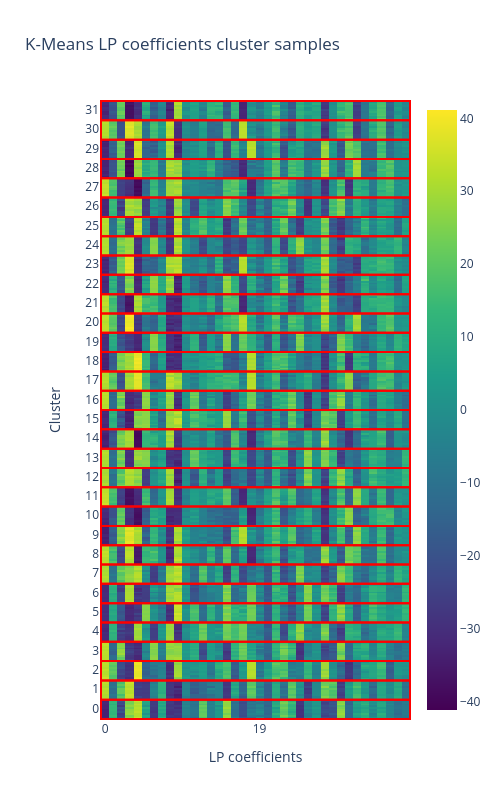
\includegraphics[width=0.22\textwidth]{mdid-5mlpcoefficientsK-Meansgridclusters.png}}
			\hspace{\fill}
			\subfloat[Output fluxes]{%
				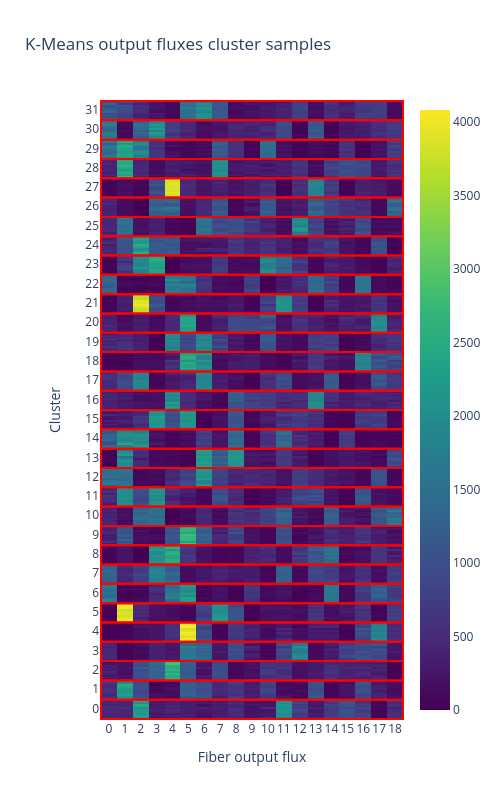
\includegraphics[width=0.22\textwidth]{mdid-5moutputfluxesK-Meansgridclusters.png}}
			\hspace{\fill}
			\subfloat[PCA PSF Intensities]{%
				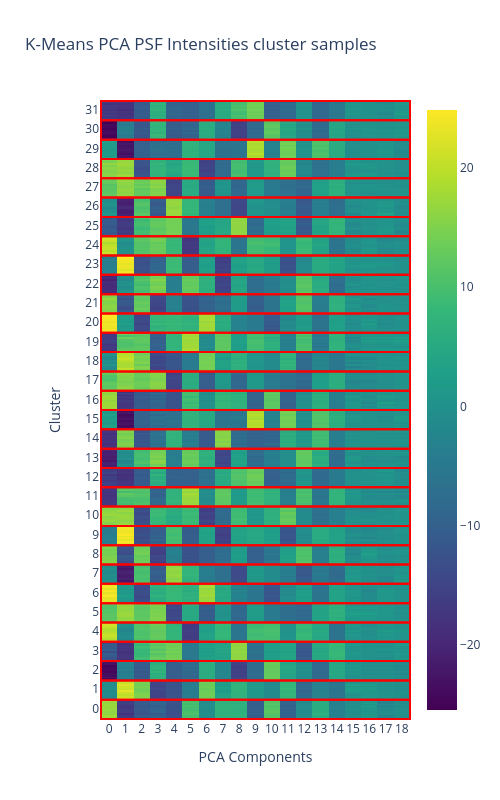
\includegraphics[width=0.22\textwidth]{mdid-5mpcaintensitiesK-Meansgridclusters.png}}
			\hspace{\fill}
			\caption{K-Means clusters from the datasets}
		\end{figure*}
		\FloatBarrier
		
		\begin{figure*}[ht!]
			\centering
			\subfloat[Zernike coefficients]{%
				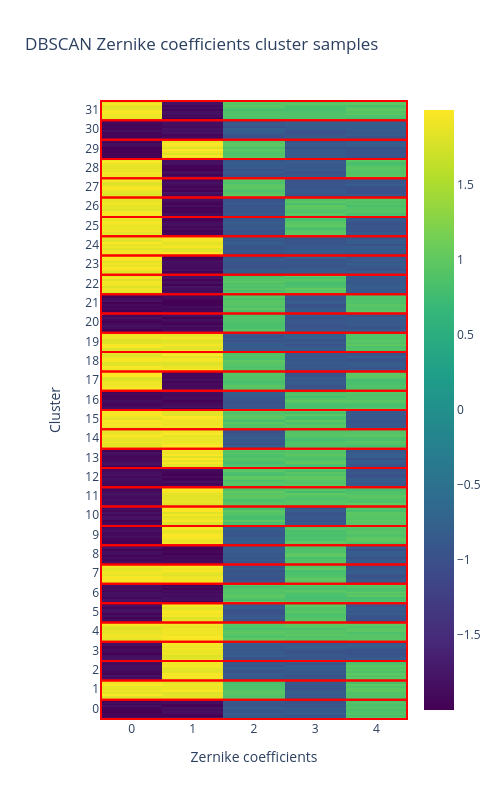
\includegraphics[width=0.22\textwidth]{mdid-5mzernikecoefficientsDBSCANgridclusters.png}}
			\hspace{\fill}
			\subfloat[LP coefficients]{%
				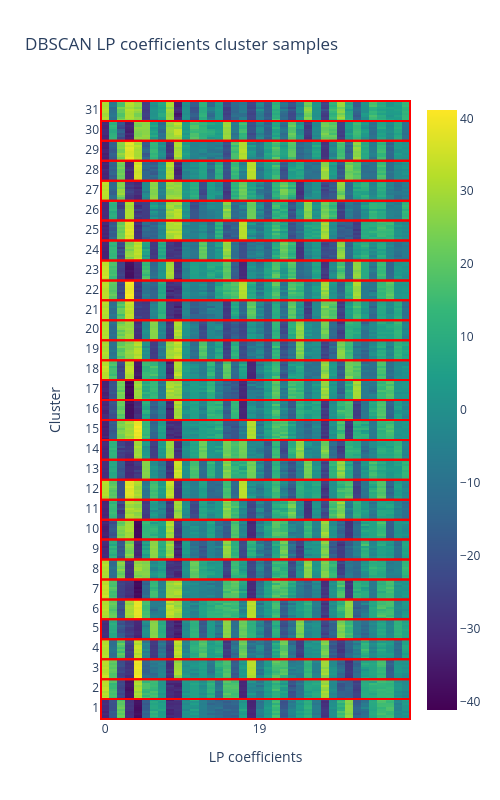
\includegraphics[width=0.22\textwidth]{mdid-5mlpcoefficientsDBSCANgridclusters.png}}
			\hspace{\fill}
			\subfloat[Output fluxes]{%
				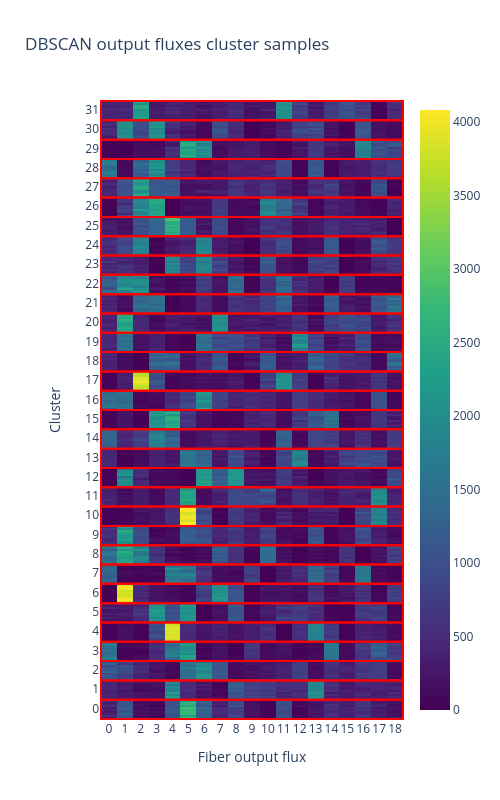
\includegraphics[width=0.22\textwidth]{mdid-5moutputfluxesDBSCANgridclusters.png}}
			\hspace{\fill}
			\subfloat[PCA PSF Intensities]{%
				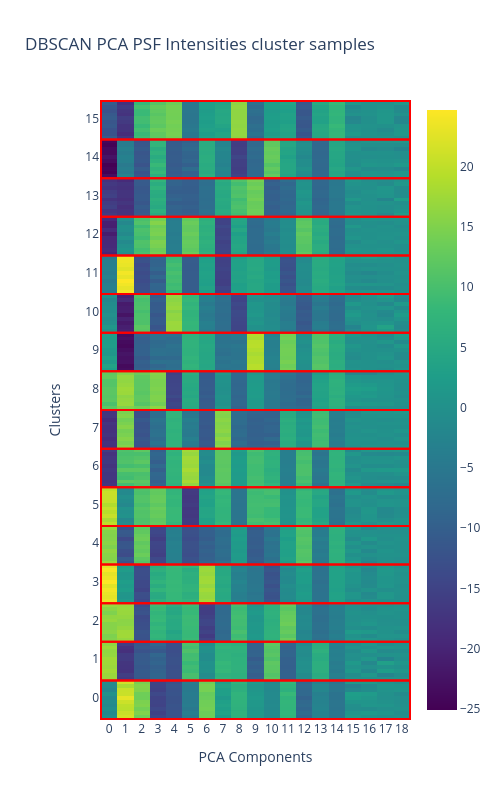
\includegraphics[width=0.22\textwidth]{mdid-5mpcaintensitiesDBSCANgridclusters.png}}
			\hspace{\fill}
			\caption{DBSCAN clusters from the datasets}
		\end{figure*}
		\FloatBarrier
		
		\begin{figure*}[ht!]
			\centering
			\subfloat[Zernike coefficients]{%
				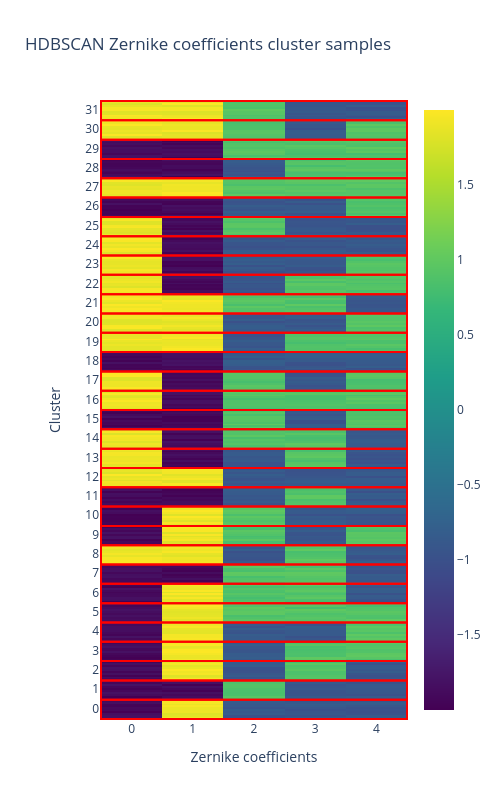
\includegraphics[width=0.22\textwidth]{mdid-5mzernikecoefficientsHDBSCANgridclusters.png}}
			\hspace{\fill}
			\subfloat[LP coefficients]{%
				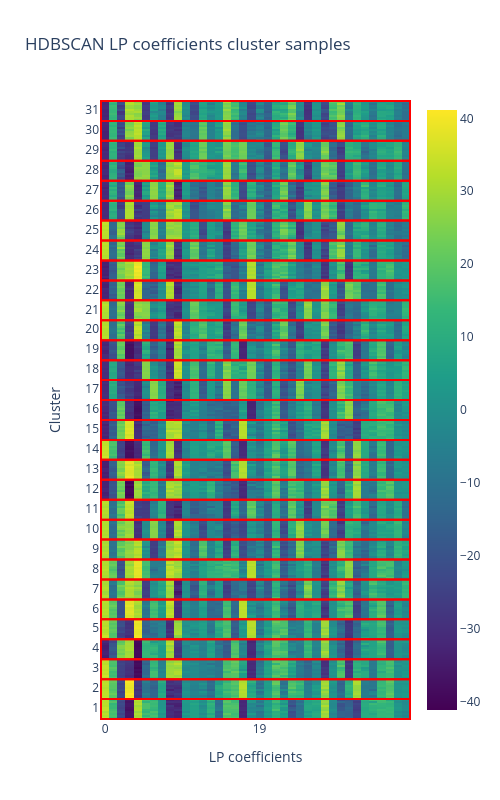
\includegraphics[width=0.22\textwidth]{mdid-5mlpcoefficientsHDBSCANgridclusters.png}}
			\hspace{\fill}
			\subfloat[Output fluxes]{%
				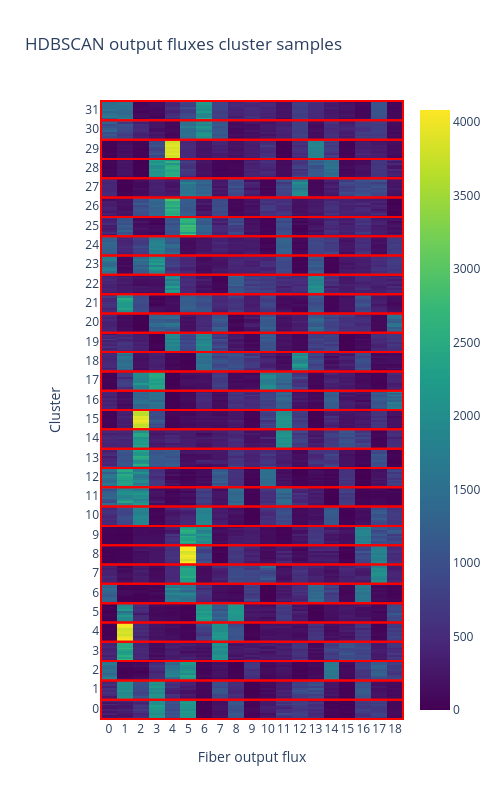
\includegraphics[width=0.22\textwidth]{mdid-5moutputfluxesHDBSCANgridclusters.png}}
			\hspace{\fill}
			\subfloat[PCA PSF Intensities]{%
				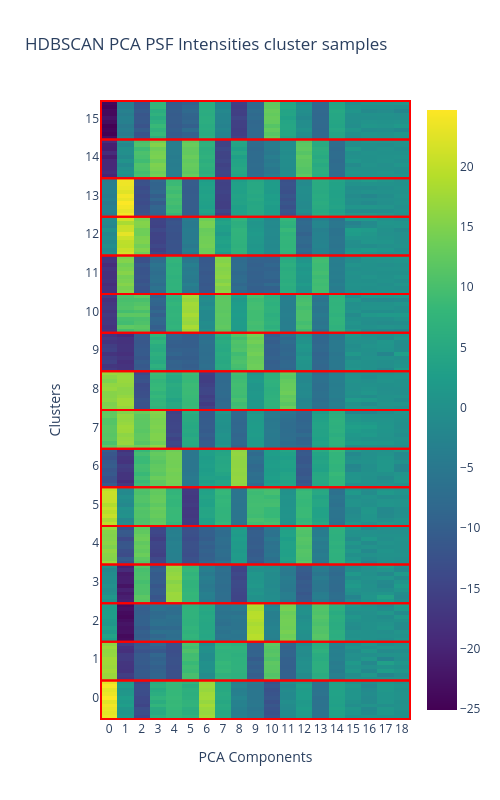
\includegraphics[width=0.22\textwidth]{mdid-5mpcaintensitiesHDBSCANgridclusters.png}}
			\hspace{\fill}
			\caption{HDBSCAN clusters from the datasets}
		\end{figure*}
		\FloatBarrier
		
		\begin{figure*}[ht!]
			\centering
			\subfloat[Zernike coefficients]{%
				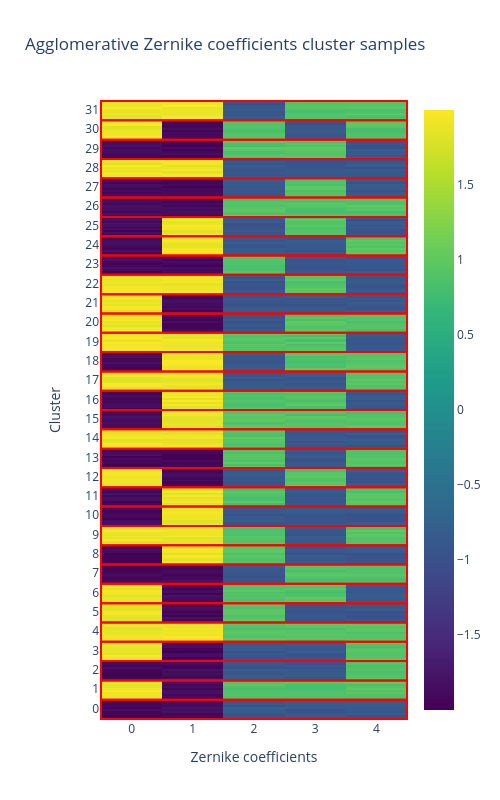
\includegraphics[width=0.22\textwidth]{mdid-5mzernikecoefficientsAgglomerativegridclusters.png}}
			\hspace{\fill}
			\subfloat[LP coefficients]{%
				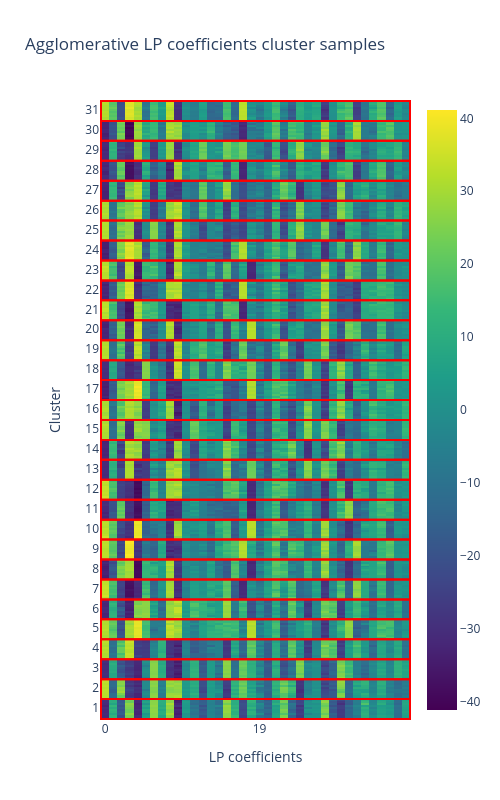
\includegraphics[width=0.22\textwidth]{mdid-5mlpcoefficientsAgglomerativegridclusters.png}}
			\hspace{\fill}
			\subfloat[Output fluxes]{%
				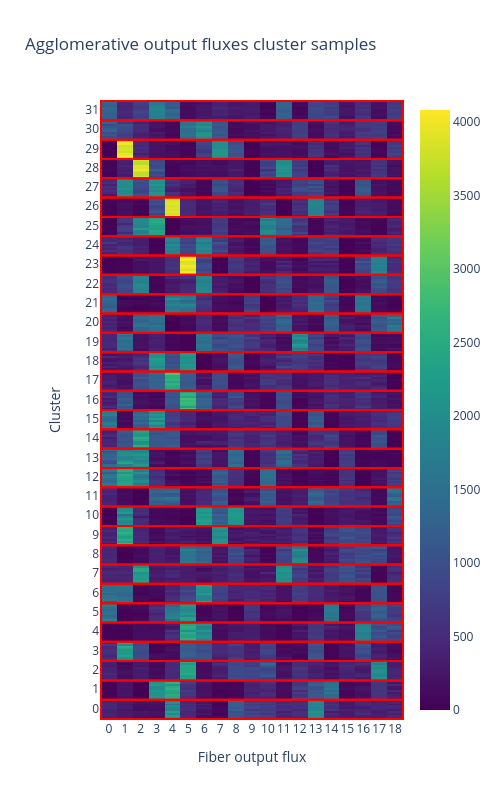
\includegraphics[width=0.22\textwidth]{mdid-5moutputfluxesAgglomerativegridclusters.png}}
			\hspace{\fill}
			\subfloat[PCA PSF Intensities]{%
				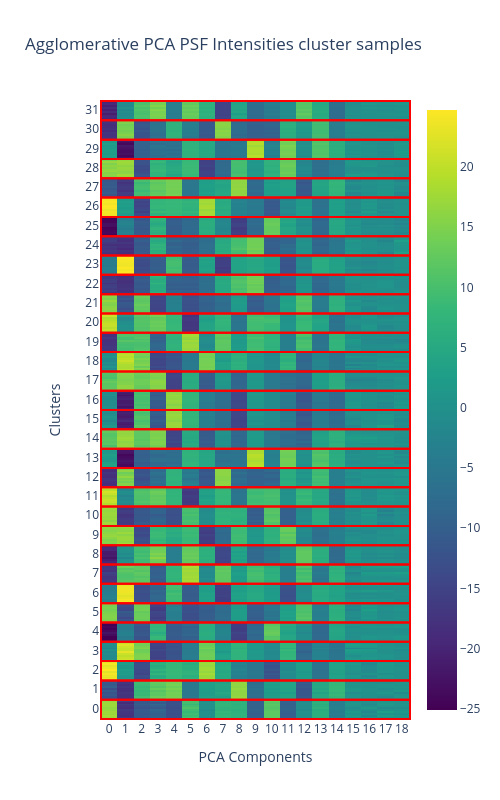
\includegraphics[width=0.22\textwidth]{mdid-5mpcaintensitiesAgglomerativegridclusters.png}}
			\hspace{\fill}
			\caption{Agglomerative clusters from the datasets}
		\end{figure*}
		\FloatBarrier